\documentclass[10pt,twocolumn,letterpaper]{article}
\usepackage[margin=0.75in,columnsep=0.25in]{geometry}
\usepackage[T1]{fontenc}
\usepackage{newtxtext,newtxmath}
\usepackage{graphicx,booktabs,amsmath,microtype,xcolor}
\usepackage[numbers,sort&compress]{natbib}
\usepackage{enumitem}
\usepackage{caption,balance,etoolbox}
\usepackage[hidelinks]{hyperref}
\usepackage{xurl}
\captionsetup{font=small,labelfont=bf,skip=5pt,hypcap=false}
\setlist[itemize]{leftmargin=*,nosep,topsep=3pt}
\setlength{\parindent}{1em}
\setlength{\parskip}{0pt}
\setlength{\textfloatsep}{11pt plus 2pt minus 2pt}
\setlength{\floatsep}{9pt plus 2pt minus 2pt}
\setlength{\intextsep}{9pt plus 2pt minus 2pt}
\newcommand{\model}{SpatialNet}
\newcommand{\pacc}[1]{P@#1}
\newcommand{\tFive}[1]{\textcolor{red}{\textbf{T5---real multi-hand evaluation.} #1}}
\newcommand{\tbd}[1]{\textcolor{red}{[#1]}}
\newcommand{\R}{\mathbb{R}}
\title{\vspace{-1.5em}\textbf{SpatialNet: Compact Pointing-Target Localisation\\for Smart Glasses with Wearer-Aware Hand Ownership}}
\author{Anonymous submission}
\date{}
\begin{document}
\raggedbottom
\twocolumn[{
\begin{minipage}{\textwidth}
\centering
{\LARGE\bfseries SpatialNet: Compact Pointing-Target Localisation\\for Smart Glasses with Wearer-Aware Hand Ownership\par}
\vspace{8pt}
{\normalsize Anonymous submission\par}
\vspace{10pt}
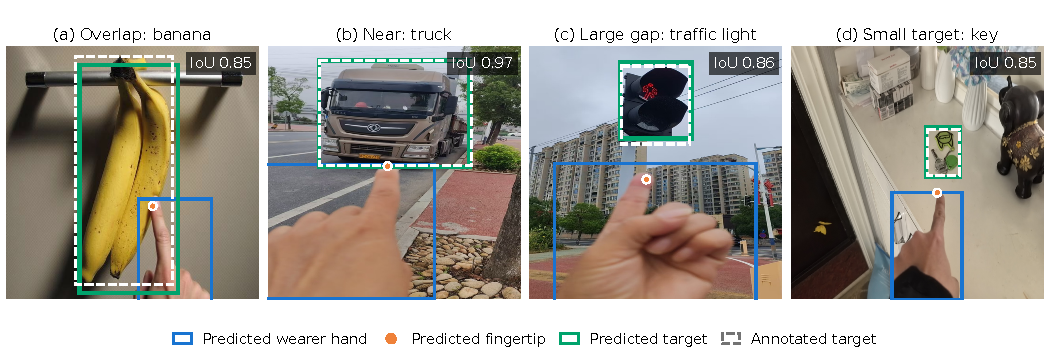
\includegraphics[width=\textwidth]{figures/teaser.pdf}
\captionof{figure}{Selected successful predictions from the EgoPoint test split, illustrating overlap (a), a nearby target (b), a larger image-plane gap (c), and a small target (d). Green: predicted target; white dashed: annotated target; blue: predicted wearer hand; orange: predicted fingertip. Boxes, points and IoUs come from the saved 160-pixel model evaluation. Original source images are displayed in the model's normalised square coordinates. These deliberately selected successes illustrate capability, not average accuracy; difficult failures appear in Figure~\ref{fig:qualitative}.}
\label{fig:teaser}
\vspace{12pt}
\end{minipage}
}]
\begin{abstract}
Pointing tells an egocentric assistant which object a request such as \emph{what is that?} refers to. Recent pointing-grounding methods resolve this reference with large vision--language backbones, up to multimodal language models with billions of parameters. Models at that scale exceed the memory and energy budgets of smart glasses, a device class whose shipments are growing rapidly, so the spatial step of the interaction is typically delegated to the cloud. We ask how much pointing-target localisation a model small enough to run on the glasses can provide, and which mechanisms matter at that scale. We present SpatialNet, a 722K-parameter, image-only convolutional network that predicts the wearer's hand, fingertip, image-plane direction and target box in one forward pass. Instance-conditioned heads share one feature map, and distractor-hand augmentation teaches the model to keep the wearer's hand as the reference. On 2,604 target-positive EgoPoint test images, SpatialNet achieves 59.0$\pm$0.1\% target \pacc{0.5} over three training seeds, with 0.23 counted GFLOPs and 1.6\,MiB of FP16 weights; prototype glasses record 60--80\,ms inference. Under their own published protocols, general-purpose 7--8B multimodal models reach 44.5--63.6\% \pacc{0.5} zero-shot or after supervised fine-tuning, and the reinforcement-trained PointVG-R reaches 83.6\%; SpatialNet uses roughly $10^4$ times fewer parameters and no text or hand-box input. Compact detectors trained under our protocol at the same computation reach 59.9--67.6\% \pacc{0.5} with 1.6--3.5 times the parameters and draw tighter boxes, but SpatialNet places its box centre on the annotated object at least as often (84.8\% against 81.6--82.9\%) and is the only model whose accuracy does not fall under synthetic hand interference. Ablations show that instance conditioning improves hand-box and direction precision, distractor training improves synthetic multi-hand robustness, and 320-pixel input raises \pacc{0.5} to 65.1\% at unchanged parameter count, whereas explicit ray conditioning does not help. Reliable hand localisation does not yet imply reliable target selection when fingertip and object are separated.
\end{abstract}
\section{Introduction}

Visual grounding links a referring expression to the image region it denotes, and it underlies how an assistant connects a user's words to the visible world~\cite{kazemzadeh2014referitgame,liu2024grounding,peng2023kosmos,you2024ferret}. In physical interaction, however, language alone often underdetermines the referent. A request such as \emph{what is that?} contains no description to match, and a cluttered scene may hold several objects that fit any short phrase. People resolve this ambiguity by pointing. Interfaces have combined pointing with speech since \emph{Put-That-There}~\cite{bolt1980put}, and embodied reference understanding now models gesture jointly with language~\cite{chen2021yourefit,li2023touchline}. Pointing-target localisation isolates the spatial core of the problem: given an image that contains a pointing hand, return the region of the indicated object. In egocentric views it is the first step of a gesture-aware assistant, which must establish where the wearer is pointing before it can recognise the object or answer a question about it~\cite{egopoint,choi2026hint,li2026egopointbench}.

Smart glasses are the setting in which this capability is most directly needed. A head-mounted camera shares the wearer's viewpoint, so the pointing hand and the indicated object can be observed in a single frame. The device category is also expanding quickly. IDC reports that worldwide extended-reality shipments grew 44.4\% in 2025, driven primarily by smart glasses, and that glasses without displays already account for the majority of those shipments~\cite{idc2026xr}. Counterpoint Research reports a 263\% year-over-year increase in AI-glasses shipments in the first half of 2026, with display-less models making up 96\% of the total~\cite{counterpoint2026aiglasses}. The growing form factor is therefore a lightweight frame that carries a camera but leaves little room for a battery or for heat dissipation. Most commercial smart glasses carry 200--300\,mAh batteries, less than one twentieth of a typical smartphone's capacity, and sustained computation on them is limited by both battery and thermal budgets~\cite{yuan2026aiglasses}. A full-system power model of an always-on research wearable likewise identifies weight and battery restrictions as the source of stringent power constraints~\cite{lee2025aria2}.

Recent pointing-grounding methods have raised accuracy substantially by building on large vision--language backbones. SV-CoT instantiates visual chain-of-thought inference on Qwen3-VL~\cite{egopoint}; PointVG-R fine-tunes a 7B-parameter Qwen2.5-VL model with chain-of-thought supervision and reinforcement learning~\cite{li2026pointvgr}; and VistaRef adds explicit hand and ray modelling to a BEiT-3 vision--language model whose base variant has 226M parameters~\cite{li2026vistaref}. Without such task-specific training, general-purpose multimodal large language models (MLLMs) remain unreliable on pointing: they often select objects near the hand or visually salient objects instead of the object the gesture indicates~\cite{li2026egopointbench,choi2026hint}. Models at the billion-parameter scale also exceed what current wearable processors can execute~\cite{yuan2026aiglasses}. The 16-bit weights of a 7B-parameter model alone occupy about 14\,GB. Liu et al.~\cite{liu2024mobilellm} note that smartphones offer 6--12\,GB of DRAM, that one application should use no more than about a tenth of it, and that a 7B model is prohibitively expensive on a phone even with 8-bit weights. Glasses have far smaller energy reserves than phones, and current smart-glasses assistants accordingly run lightweight inference locally while delegating multimodal foundation models to the cloud~\cite{yuan2026aiglasses}. Delegating pointing resolution in this way makes the most basic spatial step of the interaction depend on connectivity, adds a network round trip to every query and sends the egocentric frame off the device.

These observations define the question this paper addresses. The pointing-grounding methods above report accuracy for models with hundreds of millions to billions of parameters that also consume a text instruction and, in some settings, an externally supplied hand box~\cite{egopoint}. Sub-million-parameter networks have run on smart-glasses hardware for generic object detection~\cite{moosmann2024tinyissimoyolo}, but generic detection does not decide which object a gesture refers to. We therefore ask \emph{how much pointing-target localisation an image-only model with fewer than one million parameters can provide, and which mechanisms matter at that scale.} Answering it requires more than finding a finger. Egocentric frames can contain hands other than the wearer's~\cite{bambach2015lending}, so the model must anchor its prediction on the wearer's hand. The target box must also capture the referred object's extent, which a fingertip location alone does not determine (Section~\ref{sec:results}). A small model need not replace semantic reasoning. It can pass a target region to a recogniser or assistant while keeping the initial spatial interpretation on the device, a role that is useful only if its accuracy, failure modes and implementation cost are made explicit.

We investigate this question with \model{}, a 722,104-parameter convolutional network that predicts the wearer's hand, fingertip, image-plane direction and target box from a single RGB frame in one forward pass. A shared multi-scale feature map supports the sequence of predictions, and later heads receive features sampled around the selected hand instance rather than only a whole-image descriptor. This structure encodes the dependency of the target on the hand without a separate hand detector or pose estimator. During training, pasted hands act as distractors: the original wearer and target remain the positive reference, and the hand heatmap is penalised for responding to the added hands. Figure~\ref{fig:teaser} shows successful predictions across distinct target configurations.

On the 2,604 target-positive EgoPoint test images, \model{} reaches 59.0$\pm$0.1\% target \pacc{0.5} across three training seeds at $160\times160$ input, with 0.23 counted GFLOPs and 1.6\,MiB of FP16 weights. On prototype glasses, the deployed checkpoint recorded 60--80\,ms inference per frame. Table~\ref{tab:main} places this operating point beside published large models. With roughly $10^4$ times fewer parameters than 7--8B MLLMs, and without a text instruction or a supplied hand box, \model{} falls within the 44.5--63.6\% \pacc{0.5} range reported for general-purpose 7--8B MLLMs used zero-shot or after supervised fine-tuning~\cite{li2026pointvgr}. The compactness has a measurable cost. PointVG-R reports 83.6\% \pacc{0.5}, and the gap widens at the stricter threshold (74.5\% versus 31.5\% \pacc{0.7}). Because the published results use different inputs and evaluation populations, they locate an accuracy regime rather than establish a controlled ranking.

Controlled experiments show that the design choices matter in distinct ways. Removing the instance-conditioned pathway leaves \pacc{0.5} nearly unchanged but reduces target \pacc{0.7} by 2.8 percentage points. Removing distractor training reduces target accuracy by 4.1 points in a synthetic multi-hand stress test. Raising the input to 320 pixels increases \pacc{0.5} to 65.1\% at unchanged parameter count but about four times the counted computation. The evidence also revises an appealing geometric hypothesis: supplying the target head with an explicit ray representation does not improve its localisation after retraining, although removing that branch from an already trained network does affect its predictions. Finally, 69.0\% of target-positive test images place the annotated fingertip \emph{inside} the target box. This is image-plane overlap, not evidence of physical contact, and success on these images must not obscure the lower accuracy when fingertip and target are separated.

Our contributions are:
\begin{itemize}
\item An image-only, single-pass pointing-target localiser for smart glasses that integrates instance-conditioned prediction and wearer-specific distractor supervision within a 722K-parameter CNN, roughly four orders of magnitude smaller than the 7--8B MLLMs reported on this task.
\item A controlled evaluation of localisation precision, input resolution and synthetic hand interference, with three full-model training seeds and four targeted ablations, reported beside published large-model results with their protocol differences stated.
\item An evidence-based account of the design's limits: explicit ray conditioning is not beneficial under the tested recipe, and greater image detail improves localisation without resolving the ambiguity of separated targets.
\end{itemize}
A prototype deployment connects this operating point to smart-glasses inference. We report its observed latency separately from benchmark accuracy and do not infer interaction quality or production battery life from it.

\section{Related Work}
\paragraph{Pointing as a spatial reference.}
Gesture-based interfaces have long used pointing to connect language to visible objects~\cite{bolt1980put}. Egocentric pointing systems combine finger localisation and direction estimation to support interaction~\cite{huang2016pointing,jain2019gestarlite}; embodied reference understanding also studies how gesture complements language~\cite{chen2021yourefit}. The task here is narrower than full interaction or question answering: given a single RGB frame, output a box for the object indicated by the wearer. We do not infer object identity, infer a three-dimensional pointing ray or evaluate an interaction policy.

\paragraph{Learning to ground pointing.}
EgoPoint-Ground studies referring-expression grounding with hand pointing and provides egocentric images with hand, fingertip and object annotations~\cite{egopoint}. VistaRef develops a spatially aware pointing-to-object detector, while PointVG-R uses visual reasoning and reinforcement learning to improve localisation by multimodal models~\cite{li2026vistaref,li2026pointvgr}. These approaches supply important accuracy context, but their language inputs, training procedures and evaluation denominators differ from ours. We therefore use published results to locate the broad accuracy regime, rather than claim a controlled ranking against models we have not rerun. The distinguishing question is the usefulness and limitations of a sub-million-parameter, image-only front end.

\paragraph{Efficient localisation and instance conditioning.}
SpatialNet builds on established efficient components: ShuffleNetV2~\cite{ma2018shufflenet}, bidirectional feature fusion~\cite{tan2020efficientdet}, coordinate channels~\cite{liu2018coordconv} and local feature sampling related to RoIAlign~\cite{he2017mask}. Heatmap expectations provide continuous coordinates~\cite{sun2018integral}, while centre-based supervision avoids enumerating object proposals~\cite{zhou2019objects}. Our claim is not a new backbone or a new heatmap decoder in isolation. It is an integration in which a selected wearer-hand instance conditions subsequent predictions at small computational cost, tested against a variant that removes these instance inputs.

\paragraph{Synthetic supervision for ownership.}
Copy-paste augmentation creates useful variation for detection and segmentation~\cite{dwibedi2017cut,ghiasi2021simple}. Here its role is selective suppression: added hands are not new positive instances for the pointing task. Their locations instead receive stronger negative hand-heatmap supervision. This differs from learning to detect every hand. The resulting evaluation is necessarily limited by the synthetic placement distribution; we distinguish that controlled stress test from the pending real multi-hand check.

\section{SpatialNet}\label{sec:method}
\subsection{Task and design}
Given one RGB image, the model predicts the wearer-hand box $b_h$, fingertip $p$, unit image-plane direction $d$ and target box $b_t$. Boxes use normalised centre, width and height coordinates. A target is the annotated referred region, independent of object category. The output is intended to precede semantic recognition, whose cost and accuracy are outside this evaluation.

Three confidence logits represent wearer-hand presence, pointing conditional on a hand, and target presence conditional on pointing. The implementation can express four states: no wearer hand; a non-pointing wearer hand; pointing without a target; and pointing at a target. The available dataset contains only the first and last states. Consequently, this paper evaluates localisation and wearer-hand presence, not general pointing-event recognition.

Figure~\ref{fig:architecture} summarises the architecture. Its central design choice is to reuse a single feature map while making selected predictions depend on features sampled around the preceding prediction. This supplies spatially specific information without allocating a second detector. Conditioning is soft: an incorrect hand estimate can propagate, and shared features still contain surrounding context.

\begin{figure*}[t]
\centering
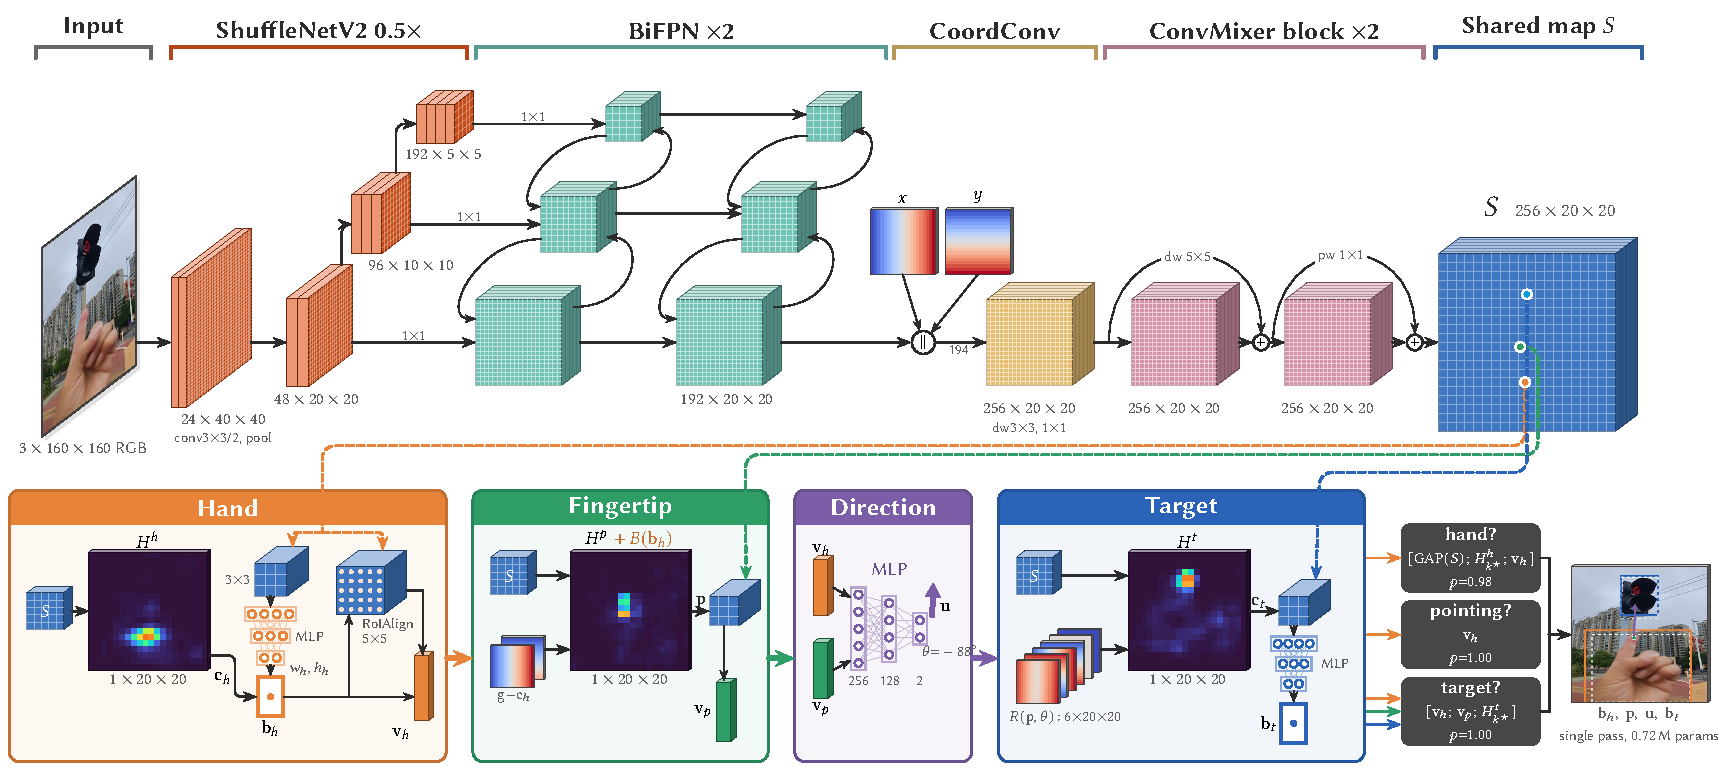
\includegraphics[width=\textwidth]{figures/architecture.pdf}
\caption{Compact instance-conditioned prediction. The hand, fingertip and target heads read the shared visual map at the previously predicted location (dashed). The selected hand supplies a box descriptor and fingertip-relative coordinates; hand and fingertip descriptors predict direction. A learned appearance-and-ray branch adds to the target heatmap, rather than restricting it to a hard cone. Local sampled features predict hand and target sizes. Distractor supervision is used only during training. The heatmaps are the trained model's outputs on one test image, overlaid on the frame and scaled to their maximum.}
\label{fig:architecture}
\end{figure*}

\subsection{Shared features and peak decoding}
A ShuffleNetV2 $0.5\times$ backbone provides stride-8, -16 and -32 features. Two bidirectional fusion layers produce 192 channels at stride 8. Depthwise smoothing with SimAM~\cite{yang2021simam}, coordinate channels and a projection to 256 channels precede two residual depthwise--pointwise mixing blocks. At 160-pixel input the shared map is $S\in\R^{256\times20\times20}$. This trunk combines local spatial detail with multi-scale context; individual component novelty is not claimed.

The hand, fingertip and target heads each predict a logit heatmap $h$. A global heatmap expectation can average distinct peaks into a location between instances. We instead take an expectation within a window $\mathcal W(k^\star)$ around the maximum-logit cell:
\begin{equation}
 \hat c=\sum_{k\in\mathcal W(k^\star)}
 \frac{\exp(\tau h_k)}{\sum_{j\in\mathcal W(k^\star)}\exp(\tau h_j)}\,g_k ,
 \quad k^\star=\arg\max_k h_k ,
 \label{eq:decode}
\end{equation}
where $g_k$ is a normalised grid coordinate. The hand and target use radius 2 and inverse temperature $\tau=8$; the fingertip uses radius 1 and $\tau=10$. Coordinates are continuous within the selected window. The discrete choice of window is not differentiable, although the expectation inside it is.

\subsection{From a hand instance to a target}
\paragraph{Hand and fingertip.}
The hand heatmap gives its centre. Bilinear sampling of a $3\times3$ neighbourhood of $S$ supports width and height regression. A $5\times5$ lattice over the predicted box, enlarged by 1.15, yields a 128-dimensional hand descriptor $v_h$. The fingertip heatmap combines a visual branch with a branch conditioned on hand-centre-relative coordinates. A soft logit penalty discourages fingertip locations outside the hand box enlarged by 1.3. The penalty uses detached box coordinates, so this prior does not push the hand box through its own gradient. A $3\times3$ neighbourhood around the decoded fingertip gives a second 128-dimensional descriptor $v_p$.

\paragraph{Direction and target.}
An MLP maps $[v_h;v_p]$ to a normalised vector $d=(d_x,d_y)$. Its target is the direction from the annotated fingertip to the annotated target-box centre, not a measured anatomical finger axis or a three-dimensional ray. This definition lets all required supervision come from the available annotation, but makes direction accuracy dependent on the chosen target extent.

The target heatmap combines visual evidence with learned spatial conditioning:
\begin{align}
 h^t_k &= V(S)_k+G([S;R(p,d)])_k, \label{eq:target}\\
 R_k &= (\Delta_x,\Delta_y,\Delta\cdot d,
              |\Delta_xd_y-\Delta_yd_x|,d_x,d_y), \nonumber\\
 \Delta &= \alpha(g_k-p). \nonumber
\end{align}
The scale $\alpha$ is learned. The final layer of $G$ starts at zero, so training begins with the visual branch alone. Both appearance features and ray-coordinate channels enter $G$; it is not a purely geometric prior. No hard constraint forces the target in front of the fingertip. The decoded target centre again anchors a $3\times3$ visual sample for box-size regression.

The hand gate receives pooled scene features, the hand heatmap peak and $v_h$. The pointing gate receives $v_h$, and the target gate receives $v_h$, $v_p$ and the target heatmap peak. At inference, sigmoid outputs are read as a cascade with threshold 0.5. This links confidence to the selected instance, but does not guarantee immunity to distractors.

\subsection{Training for localisation and ownership}
\paragraph{Localisation objective.}
Training sums masked losses for boxes, points, direction, heatmaps and gates. The hand uses CIoU~\cite{zheng2020distance}; the fingertip uses Wing loss~\cite{feng2018wing}; direction uses cosine error. The target objective combines IoU with SIoU-inspired distance and shape penalties~\cite{gevorgyan2022siou}, plus an auxiliary $1-\mathrm{IoU}$ term. The implemented distance penalty is a power of the normalised centre displacement, rather than the exponential distance term in canonical SIoU. Gaussian centre targets supervise heatmaps with a penalty-reduced focal objective, while focal binary cross-entropy supervises valid gate populations.

Two low-weight terms encourage consistency among predicted outputs. For $r=\hat c_t-\hat p$, the ray term is
\begin{equation}
 \mathcal L_{\rm ray}
 =\|r-(r\cdot\hat d)\hat d\|_2
   +0.5[-r\cdot\hat d]_+ .
 \label{eq:rayloss}
\end{equation}
The hand-axis term penalises $\max(0,0.5-\hat a\cdot\hat d)$, where $\hat a$ points from predicted hand centre to fingertip. It is a weak plausibility regulariser, not an assertion that the finger and target-centre directions always coincide. Section~\ref{sec:ablation} tests whether these losses actually improve the target box.

\paragraph{Distractor supervision.}
The released annotations do not provide positive labels for bystander hands. We therefore paste up to two hand crops into training images, keeping the original wearer/target labels. Crops may come from another image or the same wearer. Pasting is attempted with probability 0.5 on hand-positive and 0.3 on no-hand images. Scale changes and reorientation vary the appearance; crop centres are restricted to the upper 65\% of the image and overlap with labelled regions is limited. This encodes a useful but restrictive prior that the wearer hand usually enters from below.

Distractor boxes are retained to reweight negative hand-heatmap supervision. If $D_k$ is the maximum Gaussian response centred on a pasted hand, the negative weight is $1+4D_k$. The added hand is thus an explicit negative reference, even though it looks like a valid hand. This mechanism should be judged by whether localisation survives interference and whether a frame containing only other hands is rejected, rather than solely by whether a hand centre is selected correctly.

\paragraph{Optimisation and implementation.}
We use ImageNet backbone initialisation, AdamW~\cite{loshchilov2019decoupled}, batch size 32 and weight decay $10^{-4}$. A one-cycle schedule~\cite{smith2019super} peaks at $3\times10^{-3}$ for heads and $3\times10^{-4}$ for the backbone, with 10\% warm-up. Training permits 180 epochs and stops after 25 without improved validation loss; the selected checkpoint minimises that loss. Ground-truth centres replace predicted training anchors with probability 0.5, linearly decreasing to zero over 20 epochs. Other augmentations include horizontal flips, modest spatial and photometric transforms, and same-state image mixing that retains the dominant image's spatial labels. The 13 loss weights and exact target-loss definition accompany the source.

The full network has 722,104 parameters. At 160 pixels, PyTorch operation counting reports 0.231 GFLOPs with multiply--accumulate counted as two operations; unsupported operations, including bilinear sampling, are omitted. Serialised FP16 weights occupy approximately 1.6\,MiB. Weight storage and counted operations describe the model, not total runtime memory or end-to-end latency.

\section{Evaluation Protocol}\label{sec:protocol}
Our experiments answer three questions: what localisation quality is available at this model size; which design choices and input resolutions change it; and what synthetic interference tests and prototype measurements establish about deployment.

\subsection{Data and evaluation populations}
We use the released EgoPoint-Ground images~\cite{egopoint}, referred to here as EgoPoint. The release contains 10,837 training, 1,546 validation and 3,072 test images, differing from the original paper's headline counts and nominal split ratio. We preserve the released split. Its images mix real captures and generated or composed content; per-image provenance is unavailable in the conversion, so we do not claim real-only accuracy.

The deterministic conversion retains records with usable annotations, excludes positives lacking a required fingertip or hand box, and corrects three test records whose hand and object labels were swapped. The resulting training/validation/test counts are 10,669/1,524/3,029, with 9,134/1,313/2,604 target-positive images. The 425 remaining test images contain no wearer hand. The release has no annotated non-pointing-hand or pointing-without-target cases; performance of the corresponding conditional gates is therefore unestablished.

Target localisation is scored on \emph{all 2,604 positive images}, including those rejected by the confidence cascade. Thus confidence cannot improve the reported box metrics by discarding difficult examples. We report mean intersection-over-union (mIoU) and \pacc{$\tau$}, the percentage with IoU at least $\tau$. This is per-image localisation success, not detection average precision. Hand metrics use their valid annotated population; hand-presence rejection uses all relevant positive or negative images.

\paragraph{Image-plane separation.}
Let $g$ be the normalised shortest Euclidean distance from annotated fingertip to target box. We distinguish \emph{overlap} ($g=0$, 1,796 images), \emph{near} ($0<g\leq0.08$, 599), and \emph{large-gap} ($g>0.08$, 209). The coordinate system is the square-resized input. These strata concern projected annotations: overlap does not prove touching, and large gap does not prove physical distance. Their imbalance motivates reporting both pooled and stratified results.

\subsection{Comparisons and uncertainty}
The reference is the full 160-pixel, seed-42 model, also used for prototype deployment. Two retrainings use seeds 1 and 2. All runs use the same validation-selection and early-stopping rule. Training ends at different epochs; the main checkpoint is from epoch 100, while the ablation checkpoints range from 54 to 120. Consequently, ablations measure changes under a common training recipe rather than at equal optimisation steps.

Four ablations remove: (A1) hand pasting and distractor-negative weighting together; (A2) both ray and hand-axis consistency losses; (A3) the target's learned ray-coordinate branch; and (A4) instance inputs to direction/gates plus fingertip hand-offset conditioning and box prior. A4 retains local hand/target size regression and target ray conditioning. It is a bundled intervention, not a fully independent-head baseline. A3 and A4 have 708,999 and 709,191 parameters respectively.

The 224- and 320-pixel experiments retain the full architecture and seed 42. The 160/224 runs use a 224-pixel converted dataset; the 320 run is regenerated from source images at 320 pixels. The latter is therefore an increase in available image detail as well as model input resolution, not an upsampled-input experiment. No 224/320 device timings are available.

Paired image bootstrap intervals use 1,000 resamples of predictions matched by image identifier; reported 95\% percentile intervals describe test-image sampling for fixed checkpoints. They do not account for training randomness, and no multiplicity correction is applied to the exploratory comparisons. We show the three-seed full-model spread as context, not as a substitute for repeated ablation training. Published methods are listed separately because they use different inputs and incompletely specified evaluation populations.

\subsection{Synthetic hand-interference test}
A deterministic held-out transformation attempts to add one or two hands to each test image, drawing donor crops from the test split and leaving original positive labels unchanged. Successful placements occur in 2,377 of the 2,604 positive images and all 425 negatives. Evaluation uses the same transform seed across the 160-pixel ablations; donor images are never used to train these models. The target score for this condition covers all 2,604 positives, including unsuccessful placements.

We emphasise target \pacc{0.5} and rejection of no-wearer-hand frames. A centre-nearness ownership metric can saturate because the synthetic hands occupy constrained positions. This test isolates sensitivity to the specified interference distribution; real camera geometry, occlusion and social hand placement remain the scope of T5.

\section{Results}\label{sec:results}
\subsection{A compact operating point}
Table~\ref{tab:main} reports the primary result and separates it from published context. Across three training seeds, the 160-pixel model achieves 59.0$\pm$0.1\% target \pacc{0.5}, 31.5$\pm$0.4\% \pacc{0.7}, and 52.9$\pm$0.4\% mIoU (sample standard deviations). The seed-42 checkpoint reaches 58.9\% \pacc{0.5} and 53.3\% mIoU; we retain it as the reference rather than selecting a seed using test performance. Its hand \pacc{0.5} is 92.6\%, and mean fingertip error is 3.89 pixels at the 160-pixel input. Accurate hand and fingertip estimates coexist with a much larger target-localisation error.

\begin{table*}[t]
\centering
\caption{Target localisation and model scale. Accuracy entries are percentages. Our rows use all 2,604 target-positive test images; \emph{large gap} is \pacc{0.5} on the 209 images with normalised fingertip--box gap $>0.08$. Published values are contextual, not a controlled ranking: $^\ddagger$~PointVG-R~\cite{li2026pointvgr}, Table~1, uses the EgoPoint-CoT setting and does not explicitly specify no-target scoring; $^\dagger$~EgoPoint-Ground~\cite{egopoint}, Table~4, uses pointing-only grounding with a supplied hand box and an unstated evaluated subset. Published thresholds may use $>$ rather than our $\geq$. Dashes mean not reported or not applicable. Latency is the recorded glasses inference range for the 160-pixel model only.}
\label{tab:main}
\footnotesize
\setlength{\tabcolsep}{4pt}
\begin{tabular}{lrrrrrrr}
\toprule
Method / setting & Params & \pacc{0.3} & \pacc{0.5} & \pacc{0.7} & mIoU & Large gap & Latency\\
\midrule
\multicolumn{8}{l}{\emph{Published, trained on EgoPoint (not rerun)}}\\
PointVG-R$^\ddagger$, image + instruction, SFT + RL & 7B & 88.1 & 83.6 & 74.5 & 75.7 & -- & --\\
Qwen2.5-VL-7B$^\ddagger$, image + instruction, SFT & 7B & 68.7 & 63.6 & 56.7 & 59.8 & -- & --\\
\multicolumn{8}{l}{\emph{Published, zero-shot / inference-only (not rerun)}}\\
Qwen2.5-VL-7B$^\ddagger$, image + instruction & 7B & 54.2 & 49.8 & 42.9 & 45.5 & -- & --\\
Qwen3-VL-8B$^\ddagger$, image + instruction & 8B & 48.1 & 44.5 & 39.0 & 43.0 & -- & --\\
SV-CoT$^\dagger$, image + hand box & -- & 69.4 & 63.9 & 55.6 & -- & -- & --\\
Qwen3-VL-4B$^\dagger$, image + hand box & 4B & 67.1 & 61.2 & 53.2 & -- & -- & --\\
\midrule
\textbf{SpatialNet}, image only, seed 42 & 0.72M & 78.6 & 58.9 & 31.8 & 53.3 & 25.4 & 60--80\,ms\\
\quad mean $\pm$ sample std, three seeds & & $78.1\pm0.6$ & $59.0\pm0.1$ & $31.5\pm0.4$ & $52.9\pm0.4$ & $26.3\pm1.3$ & --\\
SpatialNet, 224 px input & 0.72M & 78.8 & 62.4 & 37.1 & 54.8 & 35.9 & --\\
SpatialNet, 320 px input & 0.72M & 79.4 & 65.1 & 40.3 & 56.5 & 34.9 & --\\
\bottomrule
\end{tabular}
\end{table*}

\paragraph{The box is more than a fingertip location.}
As a diagnostic reference, we place a box with mean training-set width and height at the \emph{ground-truth} fingertip. It reaches only 11.4\% \pacc{0.5}. This establishes that even an oracle fingertip is insufficient for this simple extent rule; it does not establish an upper bound for richer fingertip-conditioned methods. SpatialNet's gain reflects learning where the target centre lies and how far the referred object extends, not merely learning to find the finger.

\paragraph{Published accuracy context.}
PointVG-R reports substantially higher localisation under its protocol. The comparison also reveals why a single IoU threshold is insufficient: the zero-shot Qwen row is lower than SpatialNet at \pacc{0.5}, but higher at \pacc{0.7}. These observations motivate precision analysis; they do not establish relative superiority. The published works list a 3,072-image test split, while our conversion excludes 43 test positives and our target denominator excludes 425 negatives. Their no-target scoring is not explicit; the hand-box-assisted rows additionally use different inputs and an unstated subset. We therefore make no parity claim and do not construct a cross-hardware speedup ratio. The experimentally supported claim is the measured operating point of our own model.

\subsection{Resolution and image-plane separation}\label{sec:resolution}
Figure~\ref{fig:resolution} shows the clearest accuracy lever. At fixed parameter count, increasing input from 160 to 224 pixels raises \pacc{0.5} by 3.5 points (95\% paired interval [1.8, 5.1]); 320 pixels raises it by 6.2 points [4.4, 8.0], reaching 65.1\%. Stricter precision improves more: \pacc{0.7} rises from 31.8 to 37.1 and 40.3\%. Counted computation grows from 0.23 to 0.45 and 0.92 GFLOPs. Resolution therefore exchanges computation for accuracy without requiring more stored parameters.

\begin{figure*}[t]
\centering
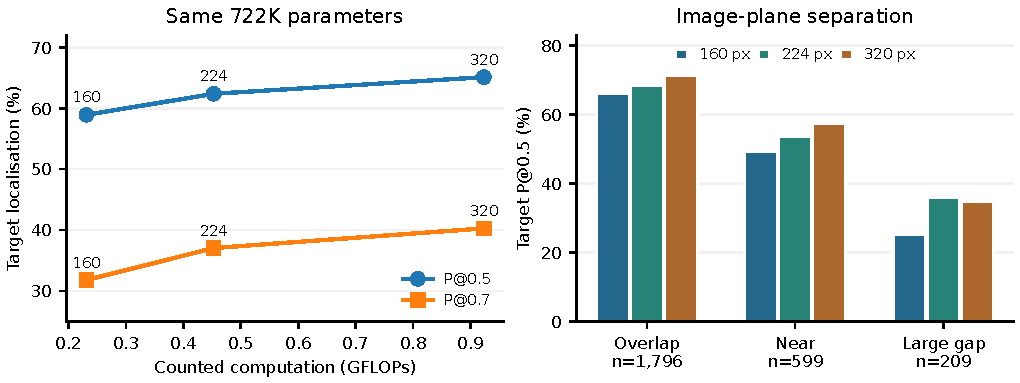
\includegraphics[width=\textwidth]{figures/resolution.pdf}
\caption{Resolution is the strongest tested accuracy lever. Left: localisation at three input sizes with the same 722K parameters; labels denote input side length. Right: \pacc{0.5} by annotated image-plane fingertip--box gap. The 320-pixel run uses source images reconverted at that resolution. Higher-resolution runs use one training seed each, and their device costs were not measured.}
\label{fig:resolution}
\end{figure*}

The strata explain what the pooled gain does and does not solve. At 160 pixels, \pacc{0.5} is 66.0\% for overlap, 49.2\% for near and 25.4\% for large-gap targets. Hand \pacc{0.5} remains approximately 93\% in all three groups. Thus, the decline cannot be explained simply by failure to find a hand. Large-gap target accuracy improves to 35.9\% at 224 pixels but is 34.9\% at 320. These single-run results show no further gain for that subset, while overall box precision continues to improve. They are consistent with unresolved reference and extent ambiguity, but do not isolate its cause or establish a resolution ceiling.

Direction also requires careful interpretation. The reference model's median angular error is 18.6 degrees against the fingertip-to-target-centre annotation. Higher resolution does not consistently reduce the mean error. Since the label itself depends on object extent, direction errors conflate geometric pointing and which target centre should be selected. Increasing spatial detail addresses part of the problem, but does not supply a separate measurement of the wearer's intended ray.

\subsection{Which design choices contribute?}\label{sec:ablation}
\begin{figure*}[t]
\centering
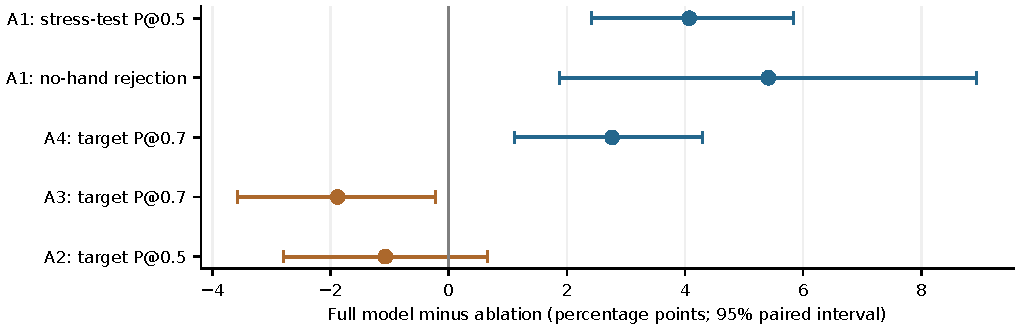
\includegraphics[width=0.93\textwidth]{figures/ablations.pdf}
\caption{Benefits are specific rather than universal. Positive values favour the full model; negative values favour removal of the component. Intervals use paired test images for the saved checkpoints, not repeated training. Distractor training helps the synthetic stress test, instance conditioning helps stricter box precision, and removing the ray branch improves that same precision metric.}
\label{fig:ablations}
\end{figure*}
Table~\ref{tab:ablations} reports every ablation's clean target \pacc{0.5} and \pacc{0.7}; Figure~\ref{fig:ablations} highlights selected mechanism-specific effects. All four changes lie within 1.1 points of the full model at \pacc{0.5}, and their paired intervals include zero. We therefore do not claim that any one component is necessary for the headline accuracy. Their differences appear in precision, auxiliary geometry and interference.

\begin{table}[t]
\centering
\caption{All four ablations, clean test set. Parameter count is in millions. A1/A2 are bundled training changes; A4 retains local box-size heads and target ray conditioning. Each variant has one training seed.}
\label{tab:ablations}
\small
\setlength{\tabcolsep}{3.5pt}
\begin{tabular}{lrrr}
\toprule
Variant & Params & \pacc{0.5} & \pacc{0.7}\\
\midrule
Full & 0.722 & 58.9 & 31.8\\
A1: no distractor training & 0.722 & 58.8 & 30.5\\
A2: no consistency losses & 0.722 & 60.0 & 32.4\\
A3: no target ray branch & 0.709 & 59.6 & 33.7\\
A4: no instance conditioning & 0.709 & 58.6 & 29.0\\
\bottomrule
\end{tabular}
\end{table}

\paragraph{Instance conditioning supports precise localisation.}
A4 reduces \pacc{0.7} by 2.8 points (full-minus-ablation interval [1.1, 4.3]) and hand mIoU by 1.8 points. Its mean direction error increases by 3.4 degrees. The reduction in target precision is larger than the 0.8-point largest \pacc{0.7} change observed between the reference and the other full-model seeds. This supports instance conditioning as a useful inductive bias under the tested recipe. It does not prove that every part of the bundled pathway is needed. A4 selected epoch 54 rather than 100, so the effect includes the training trajectory induced by that intervention.

Small targets provide supporting, less stable evidence. For boxes occupying less than 3\% of image area ($n=309$), \pacc{0.5} falls from 36.9 to 25.6\% in A4. However, the full-model seeds span 27.8--36.9\%, making this metric much more training-sensitive than the headline score. We accordingly place greater weight on the broader high-IoU and hand-box results.

\paragraph{Better direction does not imply a better target box.}
A2 removes both geometric consistency losses. Large-gap mean direction error increases by 5.6 degrees [2.1, 9.4], yet target \pacc{0.5} does not decline. This establishes a separation between improving the supervised direction and using that improvement for localisation. It provides no evidence that these losses improve the target box.

A3 offers stronger counterevidence to the original ray-conditioning hypothesis. Retraining without the target ray branch yields 59.6\% \pacc{0.5} and improves \pacc{0.7} by 1.9 points [0.2, 3.6]. The branch therefore earns no accuracy claim here. A3 selects a later checkpoint (epoch 120), and only one retraining is available, so the result should not be generalised into a universal claim against geometry.

Diagnostic interventions help interpret this outcome. On a fixed test subset, removing the branch \emph{only at inference} lowers localisation in the full trained model, whereas retraining A3 compensates for its absence. Spatial probes of the learned branch show a stronger association with proximity to the fingertip than with the signed forward ray coordinate. These findings are consistent with a proximity cue that the visual pathway can also learn. They do not prove that dataset imbalance caused this behaviour: the conditioning branch also receives appearance features, and the probe is observational. The 69\% overlap prevalence makes this a plausible explanation to investigate, not a demonstrated causal mechanism.



\subsection{Synthetic hand interference}
A1 isolates the combined effect of distractor pasting and its heatmap-negative weighting. In the synthetic stress condition, the full model reaches 60.1\% target \pacc{0.5}, compared with 56.1\% without this training. The 4.1-point paired difference has interval [2.4, 5.8]. On the 425 no-wearer-hand frames containing pasted hands, correct rejection improves from 86.4 to 91.8\%, a 5.4-point difference [1.9, 8.9]. The clean \pacc{0.5} difference is only 0.1 point, with an interval crossing zero. These results support robustness to the tested interference without a detected clean accuracy penalty.

Two cautions constrain this conclusion. First, a higher stress-test score than clean score does not mean other hands intrinsically help localisation; the transformation changes the image, and its clean-to-stress contrast is not the controlled training intervention. Second, A4 shows no clear ownership deterioration, so the evidence attributes synthetic robustness to the distractor-training package, not necessarily to instance-conditioned gates. The limited crop positions and shared train/test augmentation family also allow positional shortcuts. Real multi-hand generalisation remains unestablished.

\begin{quote}\begin{minipage}{\linewidth}\small
\tFive{Insert the real smart-glasses multi-hand check here: participant/frame counts and capture conditions; consent or ethics status and image-retention policy; wearer/target annotation and handling of disagreements; target localisation and no-wearer-hand rejection with denominators and uncertainty; and representative successes and failures. Distinguish repeated frames from independent scenes. Replace this block with the observed results and update the corresponding scope statements. No real multi-hand result is claimed in this version.}
\end{minipage}\end{quote}

\begin{figure*}[t]
\centering
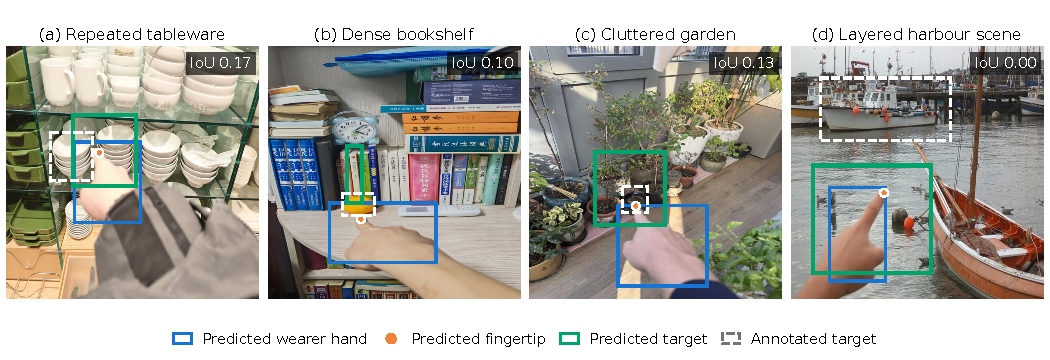
\includegraphics[width=\textwidth]{figures/qualitative.pdf}
\caption{Selected complex failures of the 722K-parameter model. Repeated tableware and dense books create neighbouring-instance ambiguity (a,b); foliage and small objects complicate target extent (c); several depth layers separate the fingertip from the labelled boat (d). Colours match Figure~\ref{fig:teaser}. Predictions and IoUs are from the saved test evaluation. These are deliberately selected hard cases, not evidence that failures occur only in complex scenes.}
\label{fig:qualitative}
\end{figure*}
\subsection{Prototype execution on smart glasses}
The 160-pixel checkpoint was deployed on a pre-production glasses unit with an onboard camera and local inference capability. The recorded engineering observations give 60--80\,ms inference per frame. This establishes execution on the prototype, but the record does not supply a latency distribution, number of repeated trials or an end-to-end timing decomposition. We therefore report the observed range rather than a percentile estimate, sustained throughput or camera-to-action response time.

The FP16 state dictionary occupies about 1.6\,MiB. A recorded additional-memory observation of approximately 100\,KB is relative to an already loaded application/model and is not total inference memory. Likewise, one-minute battery readings were 9 percentage points during continuous local inference and 16 points while streaming at 0.5 frames/s to a phone. These coarse, unmatched operating modes and the engineering power stack do not establish energy per inference, expected battery life or a general advantage over offloading. The result relevant to this paper is local feasibility at the reported latency; power and memory observations provide bounded implementation context.

\subsection{Qualitative boundary of the method}
Figure~\ref{fig:qualitative} focuses on challenging scenes with repeated objects, clutter or multiple depth layers. The tiny model selects an adjacent tableware stack or book, includes surrounding garden content, and places a foreground box instead of finding the labelled boat. These examples expose the distinction between locating a hand and resolving its reference: visual similarity and target extent remain difficult even when the hand is visible. The examples are selected to illustrate complex failures, not to estimate their prevalence or suggest that simpler scenes are error-free. Aggregate results above include every target-positive test image.



\section{Discussion and Limitations}
\paragraph{A useful front end, not complete reference understanding.}
The primary contribution is an operating point: a single compact image model can return a spatial proposal on glasses hardware. The gap between hand and target accuracy identifies the remaining difficulty. Detecting a plausible hand and fingertip is much easier than deciding which object is intended and drawing its full extent. This makes a local proposal stage a plausible component of an assistant, but its value depends on downstream tolerance for incorrect crops. Reductions in recognition cost, communication or task completion time were not measured and remain application-level implications.

The distinction between a proposal and an action is especially important for large-gap targets. Even at higher resolution, approximately two thirds of that subset fail \pacc{0.5}. A system should not treat a confident-looking box as permission for an irreversible action. Visual or verbal confirmation is a reasonable design implication, but no interaction outcome is claimed by this model evaluation.

\paragraph{Structure helps selectively.}
The ablations argue for evaluating mechanisms where they are intended to help, while still exposing the common headline metric. Instance conditioning improves stricter localisation under a common recipe; distractor supervision improves the specified interference condition; consistency losses improve a direction target without a demonstrated box benefit. The ray-branch result also prevents the architecture from being justified solely by its intuitive diagram. Learning with geometric channels is not equivalent to learning directional reasoning. A smaller A3 variant is a credible deployment candidate, but the prototype measurements and three-seed evidence belong to the full model, so we do not silently substitute the ablation as the reported system.

\paragraph{Data and generalisation.}
All quantitative model conclusions come from one released dataset, with unknown per-image provenance and incomplete demographic coverage. Its predominance of fingertip-overlap images limits what aggregate accuracy says about general pointing. The image gap is only a projected relation, and the square resize changes the geometry of non-square camera frames. Real glasses footage may differ in aspect ratio, motion blur, illumination, pose and camera--eye offset. Synthetic distractors cannot resolve these domain shifts; T5 specifically addresses real multi-hand behaviour, without turning a small check into a population-level generalisation claim.

The dataset also lacks the two conditional-negative states needed to establish general pointing and target-presence detection. A visible non-pointing hand may still trigger the cascade. Our localisation metrics do not hide these images through predicted gating, but the missing states limit deployment claims. The model predicts an image-plane target box and target-centre direction, not depth, anatomical pose or temporally coherent intent.

\paragraph{Evidence strength and reproducibility.}
Three seeds demonstrate stability of the principal full-model score, not invariance of every subgroup. Ablations and resolution variants have one seed, different stopping points and, in some cases, bundled interventions. Paired image intervals do not remove these limitations, especially for the 209 large-gap and 309 small-target examples. Published comparisons are useful context but cannot support claims of controlled superiority. The repository provides preprocessing, model/training code, variant configurations, checkpoints and per-image predictions; the accompanying audit script reconstructs the selected numerical summaries from these outputs.

\paragraph{Privacy and data practice.}
Local inference can keep the spatial-selection step on the glasses, but does not by itself make a head-worn camera private. A target crop may still contain bystanders, screens or identifying content. Consent, visible recording indication, retention limits and downstream data handling remain application responsibilities. EgoPoint is used under the authors' research-access terms; source images require separate access. The preprocessing code and evaluation outputs support reconstruction without making unrestricted redistribution of the source dataset part of the contribution. Consent and handling of new real frames are included in the T5 block.

\section{Conclusion}
SpatialNet demonstrates image-only pointing-target localisation with 722K parameters and reported execution on a smart-glasses prototype. Its value is a compact spatial front end whose strengths and boundaries are measured: instance conditioning improves precise boxes, distractor supervision improves synthetic interference robustness, and image detail yields the largest tested accuracy gain. Explicit ray conditioning does not establish a target-localisation benefit, and high hand accuracy does not resolve separated or ambiguous targets. The resulting evidence supports a practical design direction for local visual selection, while keeping real multi-hand validity and full interaction behaviour distinct from benchmark success.

\let\savedbibitem\bibitem
\def\bibitem[#1]#2{\ifstrequal{#2}{huang2016pointing}{\balance}{}\savedbibitem[#1]{#2}}
\bibliographystyle{unsrtnat}
\bibliography{references}
\end{document}

